\documentclass[aspectratio=169]{beamer}
\usetheme{Madrid}
\usecolortheme{default}
\usepackage{booktabs}
\usepackage{graphicx}
\usepackage{xcolor}

\title{Landslide Identification Using ML}
\subtitle{Lifecycle 1: Foundation \& Baseline Models}
\author{M.Tech Project}
\date{2026-03-18}

\begin{document}

% ---- Slide 1: Title ----
\begin{frame}
    \titlepage
\end{frame}

% ---- Slide 2: Problem Statement ----
\begin{frame}{Problem Statement}
    \begin{itemize}
        \item Landslides kill \textbf{thousands} and displace \textbf{millions} annually worldwide
        \item Current detection relies on manual interpretation of satellite imagery --- slow and subjective
        \item Post-disaster response needs \textbf{rapid, automated} identification to direct rescue operations
        \item Existing methods (NDVI thresholding, SVM on hand-crafted features) lack generalization
    \end{itemize}

    \vspace{0.5cm}
    \textbf{Goal:} Build an automated pipeline that:
    \begin{enumerate}
        \item Detects landslides from satellite images (Phase 1)
        \item Forecasts future landslide risk using historical patterns (Phase 2)
    \end{enumerate}
\end{frame}

% ---- Slide 3: Proposed Approach ----
\begin{frame}{Proposed Approach: Dual-Phase Pipeline}
    \begin{columns}
        \begin{column}{0.5\textwidth}
            \textbf{Phase 1: CNN Classification}
            \begin{itemize}
                \item Input: Satellite image
                \item Deep learning model classifies: \textit{landslide} or \textit{non-landslide}
                \item Outputs confidence score
            \end{itemize}
        \end{column}
        \begin{column}{0.5\textwidth}
            \textbf{Phase 2: HMM Forecasting}
            \begin{itemize}
                \item Input: Country + detection result
                \item Hidden Markov Model trained on historical data
                \item Outputs: type, risk probability, peak month, future forecast
            \end{itemize}
        \end{column}
    \end{columns}

    \vspace{0.5cm}
    \centering
    \textbf{Image $\rightarrow$ CNN $\rightarrow$ Landslide? $\rightarrow$ HMM $\rightarrow$ Risk Report}
\end{frame}

% ---- Slide 4: Datasets ----
\begin{frame}{Datasets}
    \textbf{Phase 1: HR-GLDD (Satellite Imagery)}
    \begin{table}
        \centering
        \small
        \begin{tabular}{lccc}
            \toprule
            \textbf{Split} & \textbf{Landslide} & \textbf{Non-Landslide} & \textbf{Total} \\
            \midrule
            Train & 616 & 1,574 & 2,190 \\
            Validation & 158 & 392 & 550 \\
            Test & 211 & 488 & 699 \\
            \bottomrule
        \end{tabular}
    \end{table}
    \small Note: Imbalanced --- 72\% non-landslide vs 28\% landslide

    \vspace{0.3cm}
    \textbf{Phase 2: NASA Global Landslide Catalog}
    \begin{itemize}
        \item 9,471 events across 141 countries (1988--2016)
        \item 112 country-level temporal sequences
    \end{itemize}
\end{frame}

% ---- Slide 5: Result 0 — AlexNet from Scratch ----
\begin{frame}{Result 0: AlexNet --- Baseline (Trained from Scratch)}
    \begin{columns}
        \begin{column}{0.5\textwidth}
            \textbf{Architecture:}
            \begin{itemize}
                \item 5 conv layers + 3 FC layers
                \item Input: 227$\times$227
                \item Parameters: $\sim$62M
                \item 30 epochs, LR = 0.0001
            \end{itemize}

            \vspace{0.3cm}
            \textbf{HMM:} 4 hidden states, 7 symbols
        \end{column}
        \begin{column}{0.5\textwidth}
            \textbf{Test Metrics:}
            \begin{table}
                \centering
                \small
                \begin{tabular}{lr}
                    \toprule
                    Accuracy & 78.54\% \\
                    Precision & 62.06\% \\
                    Recall & 74.41\% \\
                    F1-Score & 67.67\% \\
                    ROC-AUC & 85.53\% \\
                    \bottomrule
                \end{tabular}
            \end{table}
            \small 54 missed landslides, 96 false alarms
        \end{column}
    \end{columns}
\end{frame}

% ---- Slide 6: Result 1 — AlexNet Pretrained ----
\begin{frame}{Result 1: AlexNet --- Transfer Learning from ImageNet}
    \begin{itemize}
        \item Same AlexNet architecture, but \textbf{pre-trained on 1.2M ImageNet images}
        \item Final classifier layer replaced for 2-class landslide detection
        \item Accuracy: \textbf{80.11\%} (+1.57\% over r0)
    \end{itemize}

    \vspace{0.5cm}
    \textbf{Why transfer learning helps:}
    \begin{itemize}
        \item Our dataset has only 2,190 images --- too few to learn basic features from scratch
        \item ImageNet pre-training provides rich feature foundations (edges, textures, shapes)
        \item The model only needs to learn \textit{landslide-specific} patterns, not general vision
    \end{itemize}

    \vspace{0.3cm}
    \textbf{Takeaway:} Transfer learning gives a free accuracy boost with zero architectural changes.
\end{frame}

% ---- Slide 7: Result 2 — EfficientNet-B3 ----
\begin{frame}{Result 2: EfficientNet-B3 --- Modern Architecture}
    \begin{columns}
        \begin{column}{0.5\textwidth}
            \textbf{Upgrades:}
            \begin{itemize}
                \item Compound scaling (depth $\times$ width $\times$ resolution)
                \item Input: 300$\times$300 (74\% more pixels)
                \item Only $\sim$12M params (vs AlexNet's 62M)
                \item Differential LR + CosineAnnealing
            \end{itemize}
        \end{column}
        \begin{column}{0.5\textwidth}
            \textbf{Test Metrics:}
            \begin{table}
                \centering
                \small
                \begin{tabular}{lr}
                    \toprule
                    Accuracy & 79.97\% \\
                    Precision & 63.71\% \\
                    \textbf{Recall} & \textbf{78.20\%} \\
                    F1-Score & 70.21\% \\
                    ROC-AUC & 88.93\% \\
                    \bottomrule
                \end{tabular}
            \end{table}
        \end{column}
    \end{columns}

    \vspace{0.3cm}
    \textbf{Key win:} Recall jumped from 74.41\% $\to$ 78.20\% --- \textbf{8 fewer missed landslides}. \\
    In disaster monitoring, missing a landslide is far worse than a false alarm.
\end{frame}

% ---- Slide 8: Dataset Samples ----
\begin{frame}{Dataset: What the Model Sees}
    \begin{columns}
        \begin{column}{0.5\textwidth}
            \centering
            \textbf{Landslide Image}\\[0.3cm]
            
\includegraphics[width=0.75\textwidth]{project/data/processed/test/debris_flow/ls_test_0011.jpg}\\[0.2cm]
            \small Debris flow --- exposed soil, vegetation loss
        \end{column}
        \begin{column}{0.5\textwidth}
            \centering
            \textbf{Non-Landslide Image}\\[0.3cm]
            
\includegraphics[width=0.75\textwidth]{project/data/processed/test/non_landslide/nls_test_0001.jpg}\\[0.2cm]
            \small Normal terrain --- intact vegetation
        \end{column}
    \end{columns}

    \vspace{0.3cm}
    \centering
    \small The model must learn to distinguish these 128$\times$128 satellite patches
\end{frame}

% ---- Slide 9: Training Output ----
\begin{frame}{Training Output: Loss \& Accuracy Curves}
    \centering
    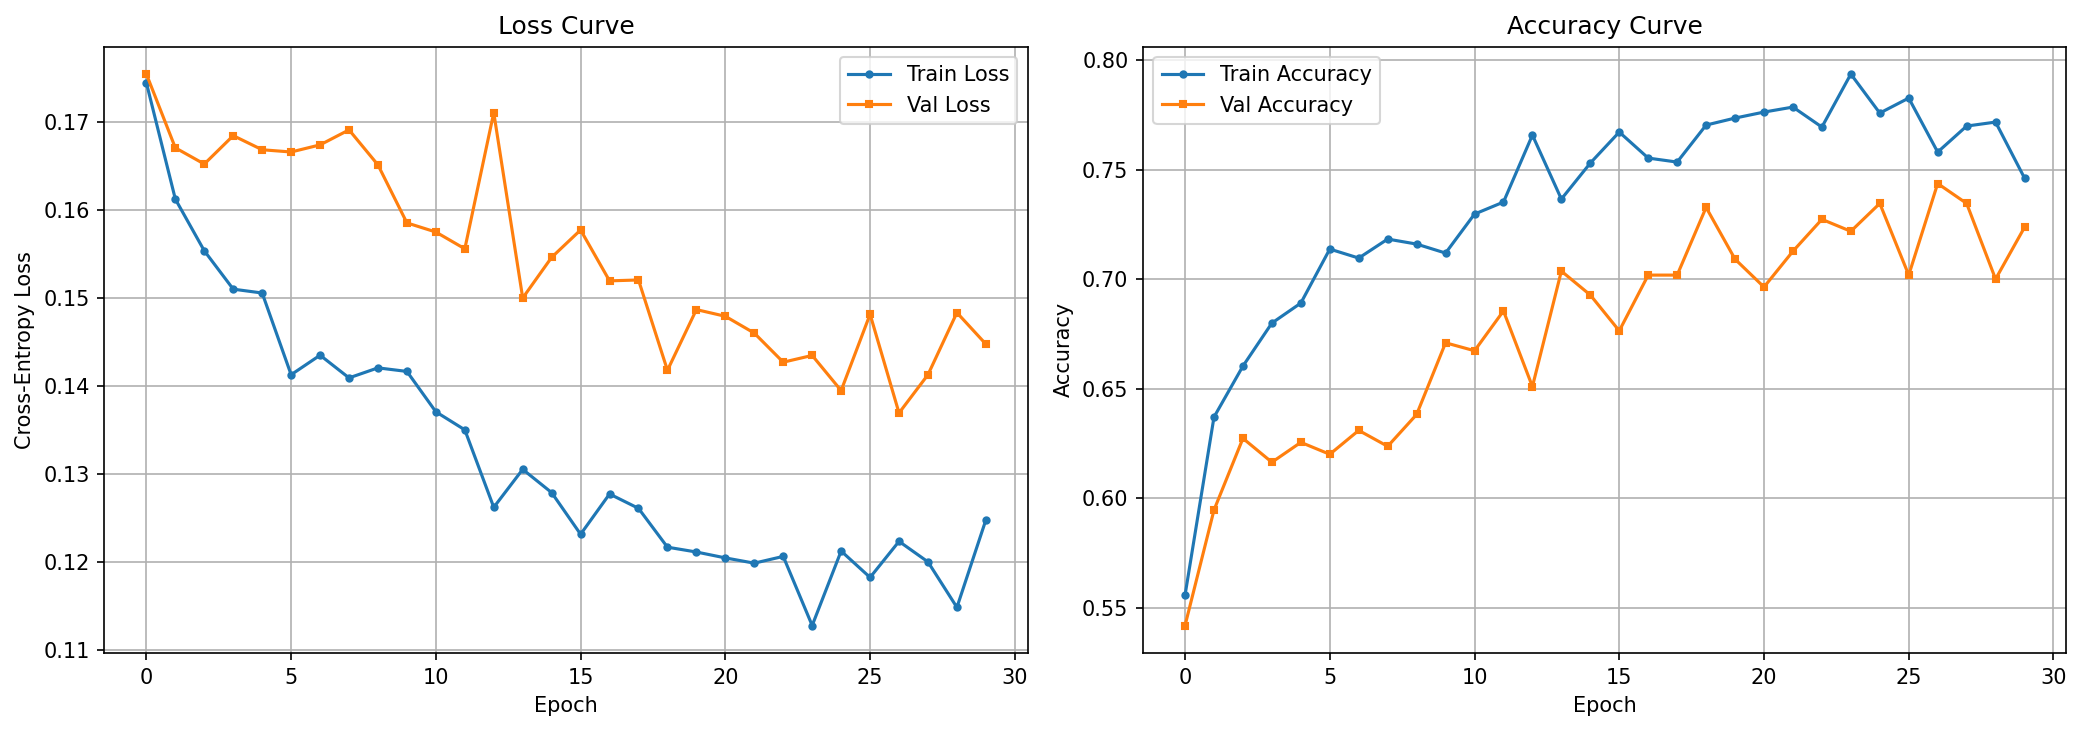
\includegraphics[width=0.85\textwidth]{project/plots/training_history.png}

    \vspace{0.2cm}
    \small Training loss decreases over epochs $\to$ model is learning.\\
    Validation accuracy plateaus $\to$ model has reached its capacity with this architecture.
\end{frame}

% ---- Slide 10: Evaluation Output ----
\begin{frame}{Evaluation Output: Confusion Matrix \& ROC Curve}
    \begin{columns}
        \begin{column}{0.5\textwidth}
            \centering
            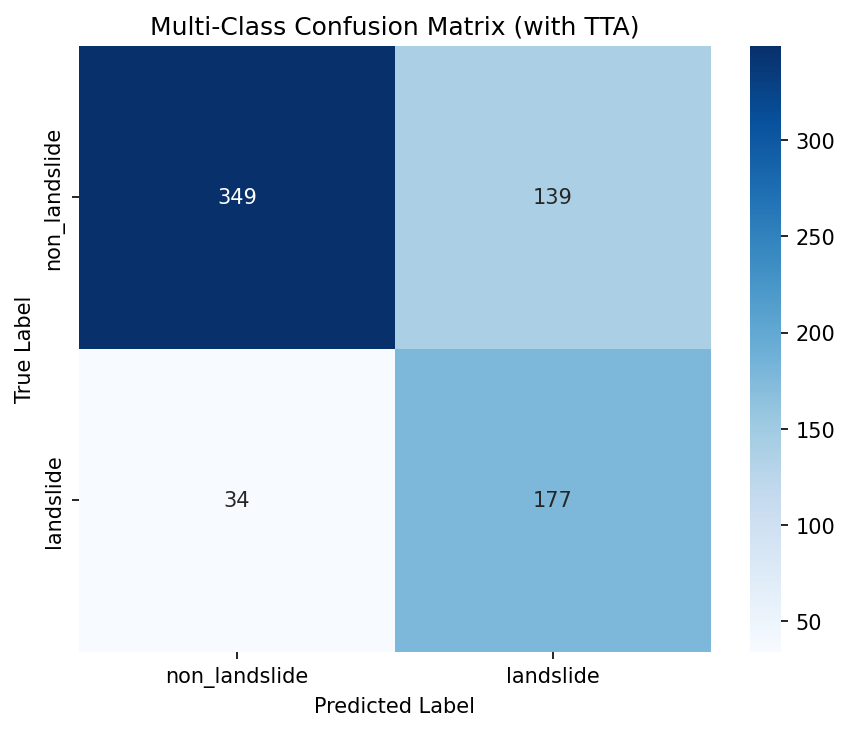
\includegraphics[width=0.95\textwidth]{project/plots/confusion_matrix.png}\\[0.1cm]
            \small Confusion Matrix --- shows TP, FP, FN, TN counts
        \end{column}
        \begin{column}{0.5\textwidth}
            \centering
            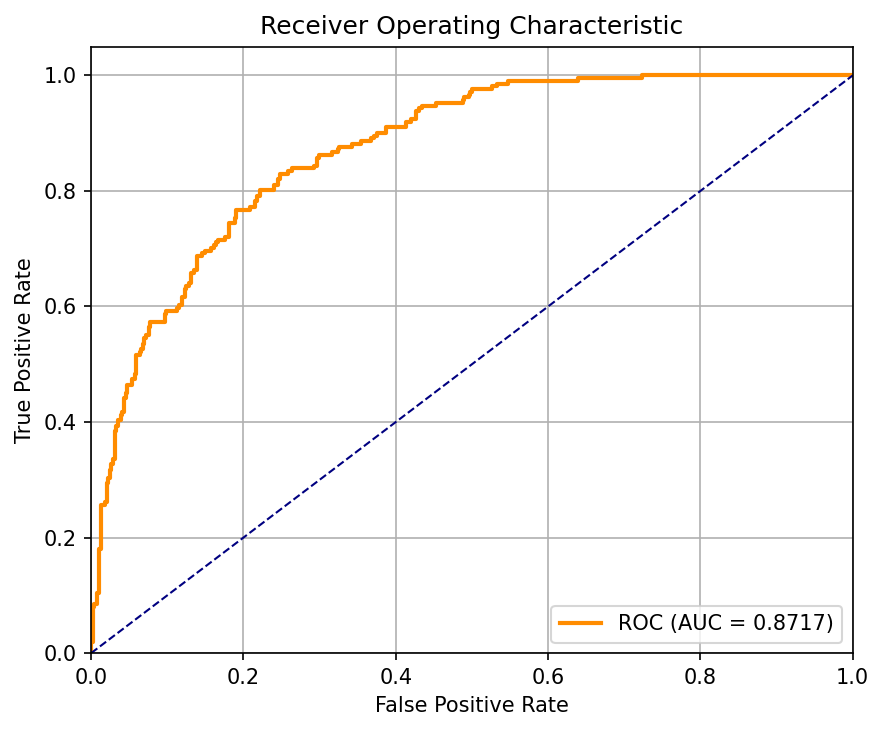
\includegraphics[width=0.95\textwidth]{project/plots/roc_curve.png}\\[0.1cm]
            \small ROC Curve --- AUC measures ranking ability
        \end{column}
    \end{columns}
\end{frame}

% ---- Slide 11: Pipeline Output ----
\begin{frame}[fragile]{Pipeline Output: Single Image Prediction}
    \textbf{Command:}
    \begin{verbatim}
python pipeline/run_pipeline.py --mode predict \
    --image data/processed/test/debris_flow/ls_test_0011.jpg \
    --country India --forecast 3
    \end{verbatim}

    \textbf{Output:}
    \begin{verbatim}
Phase 1 - LANDSLIDE (confidence: 95.9%)
Phase 2 - Type: Landslide
          Occurrence probability: 30.0%
          Peak risk month: July
          Future forecast:
            Step 1: Landslide (prob=26.4%)
            Step 2: Landslide (prob=21.4%)
            Step 3: Landslide (prob=18.1%)

LANDSLIDE DETECTED - Type: Landslide (prob: 30%)
    \end{verbatim}
\end{frame}

% ---- Slide 12: Comparison Table ----
\begin{frame}{Lifecycle 1: Results Comparison}
    \begin{table}
        \centering
        \renewcommand{\arraystretch}{1.3}
        \begin{tabular}{llccccc}
            \toprule
            \textbf{Result} & \textbf{Model} & \textbf{Acc} & \textbf{Prec} & \textbf{Rec} & \textbf{F1} & \textbf{AUC} \\
            \midrule
            r0 & AlexNet (scratch) & 78.54 & 62.06 & 74.41 & 67.67 & 85.53 \\
            r1 & AlexNet (pretrained) & 80.11 & 66.67 & 67.30 & 66.98 & 85.73 \\
            \textbf{r2} & \textbf{EfficientNet-B3} & \textbf{79.97} & \textbf{63.71} & \textbf{78.20} & \textbf{70.21} & \textbf{88.93} \\
            \bottomrule
        \end{tabular}
    \end{table}

    \vspace{0.3cm}
    \textbf{Progression:}
    \begin{itemize}
        \item F1-Score: 67.67\% $\to$ 70.21\% (+2.54\%)
        \item ROC-AUC: 85.53\% $\to$ 88.93\% (+3.40\%)
        \item False Negatives: 54 $\to$ 46 (fewer missed landslides)
    \end{itemize}
\end{frame}

% ---- Slide 9: Key Findings ----
\begin{frame}{Key Findings from Lifecycle 1}
    \textbf{Strengths:}
    \begin{itemize}
        \item Dual-phase pipeline works end-to-end (image $\to$ risk report)
        \item Transfer learning essential for small datasets
        \item EfficientNet-B3 significantly better at detecting landslides (recall)
    \end{itemize}

    \vspace{0.4cm}
    \textbf{Identified Weaknesses (to address in LC2):}
    \begin{enumerate}
        \item \textbf{Overconfident predictions} --- model says 95\% confident but is only $\sim$75\% accurate
        \item \textbf{Single model limitations} --- one architecture has systematic blind spots
        \item \textbf{Simplistic HMM} --- only observes landslide type, ignores trigger mechanisms
        \item \textbf{Arbitrary threshold} --- 50\% cutoff is not optimized
    \end{enumerate}
\end{frame}

% ---- Slide 10: LC2 Preview ----
\begin{frame}{Lifecycle 2 Preview: Optimization \& Ensemble}
    \textbf{Based on LC1 weaknesses, the next lifecycle will address:}

    \vspace{0.3cm}
    \begin{enumerate}
        \item \textbf{Temperature Scaling (Confidence Calibration)}
            \begin{itemize}
                \item Fix overconfident softmax outputs
                \item Make confidence scores reliable for operational thresholds
            \end{itemize}

        \item \textbf{Ensemble Methods}
            \begin{itemize}
                \item Combine EfficientNet-B3 + AlexNet to cancel out individual errors
                \item Explore Vision Transformer (ViT) for global spatial features
                \item Data-driven optimal threshold instead of arbitrary 50\%
            \end{itemize}

        \item \textbf{Richer HMM Observations}
            \begin{itemize}
                \item Add trigger mechanisms: type $\times$ trigger = 42 combined symbols
                \item Increase hidden states: 4 $\to$ 8 for finer regime modeling
            \end{itemize}
    \end{enumerate}
\end{frame}

% ---- Slide 15: Thank You ----
\begin{frame}{}
    \centering
    \vspace{2cm}
    {\Large \textbf{Thank You}}

    \vspace{1cm}
    Questions \& Discussion
\end{frame}

\end{document}
